% CHI Extended Abstracts template.
% Tested with XeTeX on Mac OS X (Get it from http://tug.org/mactex)
% The latest version is available at <http://manas.tungare.name/software/latex/>
% 
% Filename: chi-ext.cls
% 
% CHANGELOG:
%   2010-10-18   Manas Tungare      Restored support for \figures.
%   2010-08-09   Manas Tungare      Updated copyright info for CHI 2011
%   2009-12-04   Stephen Voida      Updated copyright info for CHI 2010
%   2008-11-25   Manas Tungare      Initial create.
%   2009-11-17   Manas Tungare      Refactored the title & author sections.
% 
% LICENSE:
%   Public domain: You are free to do whatever you want with this template.
%   If you improve this in any way, please drop me a note <manas@tungare.name>,
%   so I can share the updates with everyone.
%   
%   PLEASE RECONSIDER BEFORE FORKING THIS TEMPLATE; there are already
%   several versions of the chiproceedings template for no good reason.
%   DO NOT REDISTRIBUTE THIS FILE UNDER A DIFFERENT FILENAME unless you
%   have a very good reason to change its name.
\documentclass{chi-ext}
\parskip=2pt
\title{Design Fiction Report : NaviLens - Enabling Active Decision-Making For A Safer Future}

\author{
  \textbf{MarkChunYong Ting} \\
  University of Melbourne \\
  Student ID : 805780 \\
  Student Account : mting3 \\
  mting3@student.unimelb.edu.au \\
  \\
  \textbf{ShiXun Liu} \\
  University of Melbourne \\
  Student ID : 766799 \\
  Student Account : shixunl \\
  shixunl@student.unimelb.edu.au \\
  \\
  \textbf{MengYu Gong} \\
  University of Melbourne \\
  Student ID : 842183 \\
  Student Account : gongm1 \\
  gongm1@student.unimelb.edu.au \\
}

\keywords{Smart lenses; Navigation; Mobile Distraction; Augmented Reality; Design fiction; Safer Future; Decision-making}

\acmclassification{H.5.2 Information Interfaces and Presentation: User interfaces –
Evaluation/ methodology}

\copyrightinfo{
  Copyright is held by the author/owner(s). \\
}

% Repeat author names (minus affiliations and addresses) and title here 
% for PDF metadata.
\hypersetup{
  pdfauthor={MarkChunYong Ting, ShiXun Liu, MengYu Gong},
  pdfkeywords={Keyword 1, Keyword 2},
  pdfsubject={General Subject Area},
  pdftitle={Paper Title Goes Here},
}

\begin{document}
\maketitle

\begin{multicols}{2}
  
\makeauthors
\makecopyright

\section{Abstract}

According to Australian Road Deaths Database statistics from the Department of Transport,  the growing dependence on and the frequent interactions with mobile devices has been a major factor in fatalities. Tackling with this intractable concern, the Melbourne University CIS Research Group cooperated with the Department of Transport Australia and Melbourne Medical School, had developed an intelligent contact lens NaviLens. Using double diamond design process, Research Group adopted various user research methods such as video diary, ethnography, competitor analysis. In this paper, we present the user desirability results, the NaviLens product structure and its major functions, we also demonstrated a trial on the feasibility, viability, and effect of the NaviLens at the end.\\


\section{Keywords}
\makeatletter \@keywords \makeatother

\section{ACM Classification Keywords}
\makeatletter \@acmclassification \makeatother

%------------------------------------------------------------------------

\section{Introduction}

\subsection{Problem}
According to a recent research of Morgan Stanley analysts team over traffic fatalities in the Australia from 1921 to 2015, it is noticeable that motor vehicle deaths increased by 8\% --- or the largest percent increase in 50 years --- in 2015, according to preliminary estimates from the National Safety Council. An estimated 38,300 people were killed on Australia roads (Elena Holodny, Traffic fatalities in the US have been mostly plummeting for decades).\\

\begin{figure}
\centering
  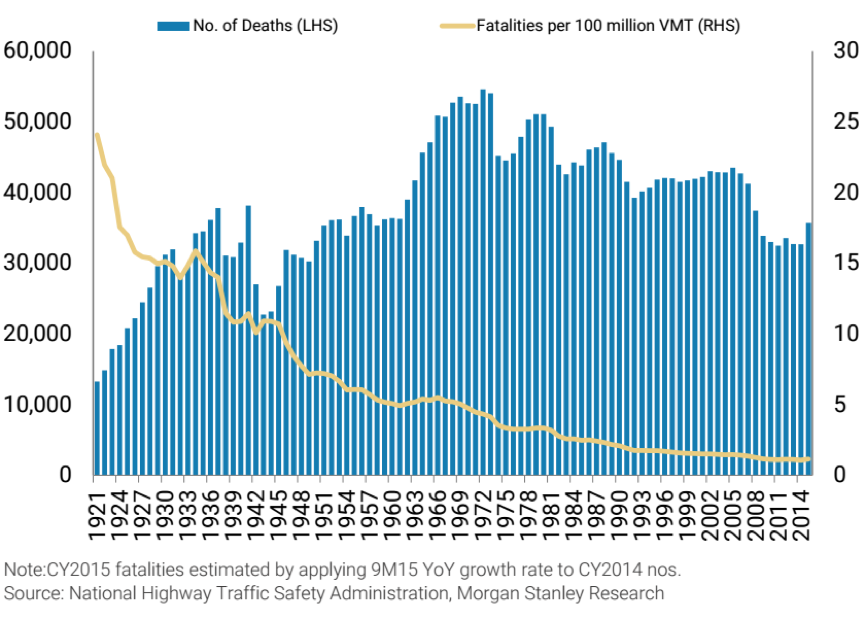
\includegraphics[width=\columnwidth]{barchart.png}
  \caption{Barchart}
 \label{fig:barchat}
\end{figure}

\subsection{Discover}
The Department of Transport Australia delegated the CIS research group to further investigate this issue, Michael Anderson, the Minister of Transport told us the number of car accidents due to mobile distractions had been constantly increasing in recent years. As shown in the following table, according to Department of Transport statistics from 2005 to 2017, there are four main reasons for car crashes, and mobile distractions occupy a major part (19\%) among them.\\ 

\begin{figure}
\centering
  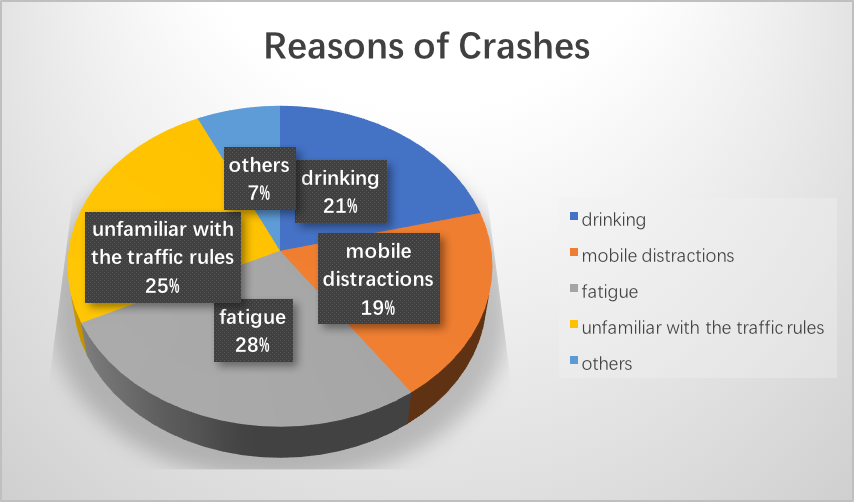
\includegraphics[width=0.7\columnwidth]{table.png}
  \caption{Table}
 \label{fig:table}
\end{figure}

We interviewed Johnson Martin a 27-years-old employee who just stepped into the workplace, he said it’s impossible to mute your phone or throw it in the bag, “it takes me one and a half hour heading office from home, I cannot miss out a working call or any emergencies, besides, I need to play something during traffic jam. There a lot of people like Johnson, Peter Tucker, a 35 years old contractor said, “I used to use car navigation, but it’s not working very well, so I just simply use Google maps on my phone, you know, it’s easy, I can also answer phones.” \\

\subsection{Define}
We had found that the burst of useful mobile apps brought us huge convenience yet the growing dependence on mobile devices had brought many potential dangers as well. The mobile devices should take considerable responsibilities of the sudden increase of traffic fatalities in 2015. Our researchers made cooperation with Department of Transport and made further investigation, we noticed that 62.3\% drivers using phones when waiting for traffic lights, 34.7\% drivers answering phones when driving, 21.1\% car owners implemented car holders to use mobile phones more conveniently, such as for navigation etc. However, drivers had to frequently remove their eyes from road condition to the phones and adjust the car holder many times during driving because sometimes it just not worked that good.\\

\subsection{Develop}

\begin{figure}
\centering
  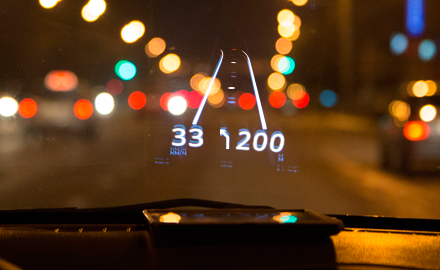
\includegraphics[width=0.7\columnwidth]{windscreen.png}
  \caption{Windscreen}
  \centering
 \label{fig:windscreen}
\end{figure}

We considered to show the navigation information on the windscreen, however, the effects are not that good for the unclear image and especially on rainy days or nights, the lights on windscreen will even disturb your sight. Admittedly, Google Glass had realized the navigation function through the lens, however, we interviewed 8 Google Glass users and 7 of them complained that it would cause dizziness whilst wearing it for a long time, which is detrimental when driving.
Chiou, Jin-Chern in his "A Wirelessly Powered Smart Contact Lens with Reconfigurable Wide Range and Tunable Sensitivity Sensor Readout Circuitry." \cite {ref1} presented a wireless smart contact lens system that was composed of a reconfigurable capacitive sensor interface circuitry and wirelessly powered radio-frequency identification (RFID) addressable system for sensor control and data communication, which provided a hardware design theory basis for us. In "Route Visualization in Indoor Panoramic Imagery with Open Area Maps"\cite {ref5}, the author demonstrated the city augmented by location information, which also gives us an inspiration of adopting augmented reality technology. \\

\subsection{Deliver}
Therefore, based on our investigation and research cooperated with the Department of Transport, we developed a new high-tech product NaviLens, aimed at reducing the dependence on mobile devices, decrease the dangers of frequent interaction with mobile devices and enable active decision-making for a safer future. NaviLens is an intelligent contact lens, whose major features are Global Positioning System, Signboard attention, functions for Eye sightedness and Color blindness, and Driving Enforcement Marking System. The Global Positioning System will show necessary navigation graph and information on Navilens, in this way drivers do not need to move their eyes from the road to other places, which reduce the mobile distractions when driving. The Signboard attention and Driving Enforcement Marking System regulate the driving habits and help drivers notice potential dangers which can reduce plenty of car accidents due to the unfamiliarity of traffic rules or fatigue. The Navilens had got the support from Department of Transport and authentication of The Royal Society of Medicine and released in Australia, in the end of June 2017, it broke into the international market and had been known and used by more and more people.\\

The Navilens instructions are as follows:
\begin{itemize}
  \item Age:18 -- 65, with no eye diseases
  \item If wearing lenses on an extended wear basis, remove and dispose of your lenses the evening before you are due to replace them, inserting new lenses the following day.
  \item	If your eyes become red or irritated or you experience any pain or unexpected change in vision, remove your lenses immediately and consult your eye-care practitioner.
  \item	For lenses worn more than once, always clean and disinfect your lenses as instructed, after lens removal.
  \item	DO NOT sleep in your lenses unless your eye-care practitioner has advised it is safe to do so.
  \item	DO NOT wear your lenses beyond the period recommended by your eye-care practitioner. 
  \item	DO NOT use household products (e.g. disinfectants) on your lenses. 
  \item	DO NOT rinse your lenses or lens case with tap water.
  \item	Keep your lenses out of the reach of children
\end{itemize}

\subsection{NaviLens Structure}

The circuit board of NaviLens contains eight parts. The main component is the micro monitors which is arranged in the array and covers the center of the board. The micro monitors use the semi-transparent material through which user will still be able to glance without affecting the eyesight while providing an extra visual feature on top. One display control unit controls these monitors. Then, NaviLens has a telecommunication chip which is used to connect with user’s mobile phone to stream the information to and from the mobile phone. The visual capture lens will capture the image or video on activation and will send out the information through the telecommunication chip. Motion sensor detects the motion of user head movement or eye movement and provides some predefined gesture function. For electricity usage, NaviLens has one large capacitor, and the electric control unit is in charge of controlling the electric usage for each component depending on the needs. The electric assumption of NaviLens is very low and can last whole day long. If needed, NaviLens can be recharged through the NaviLens Multifunction Casing.\\


\begin{figure}
 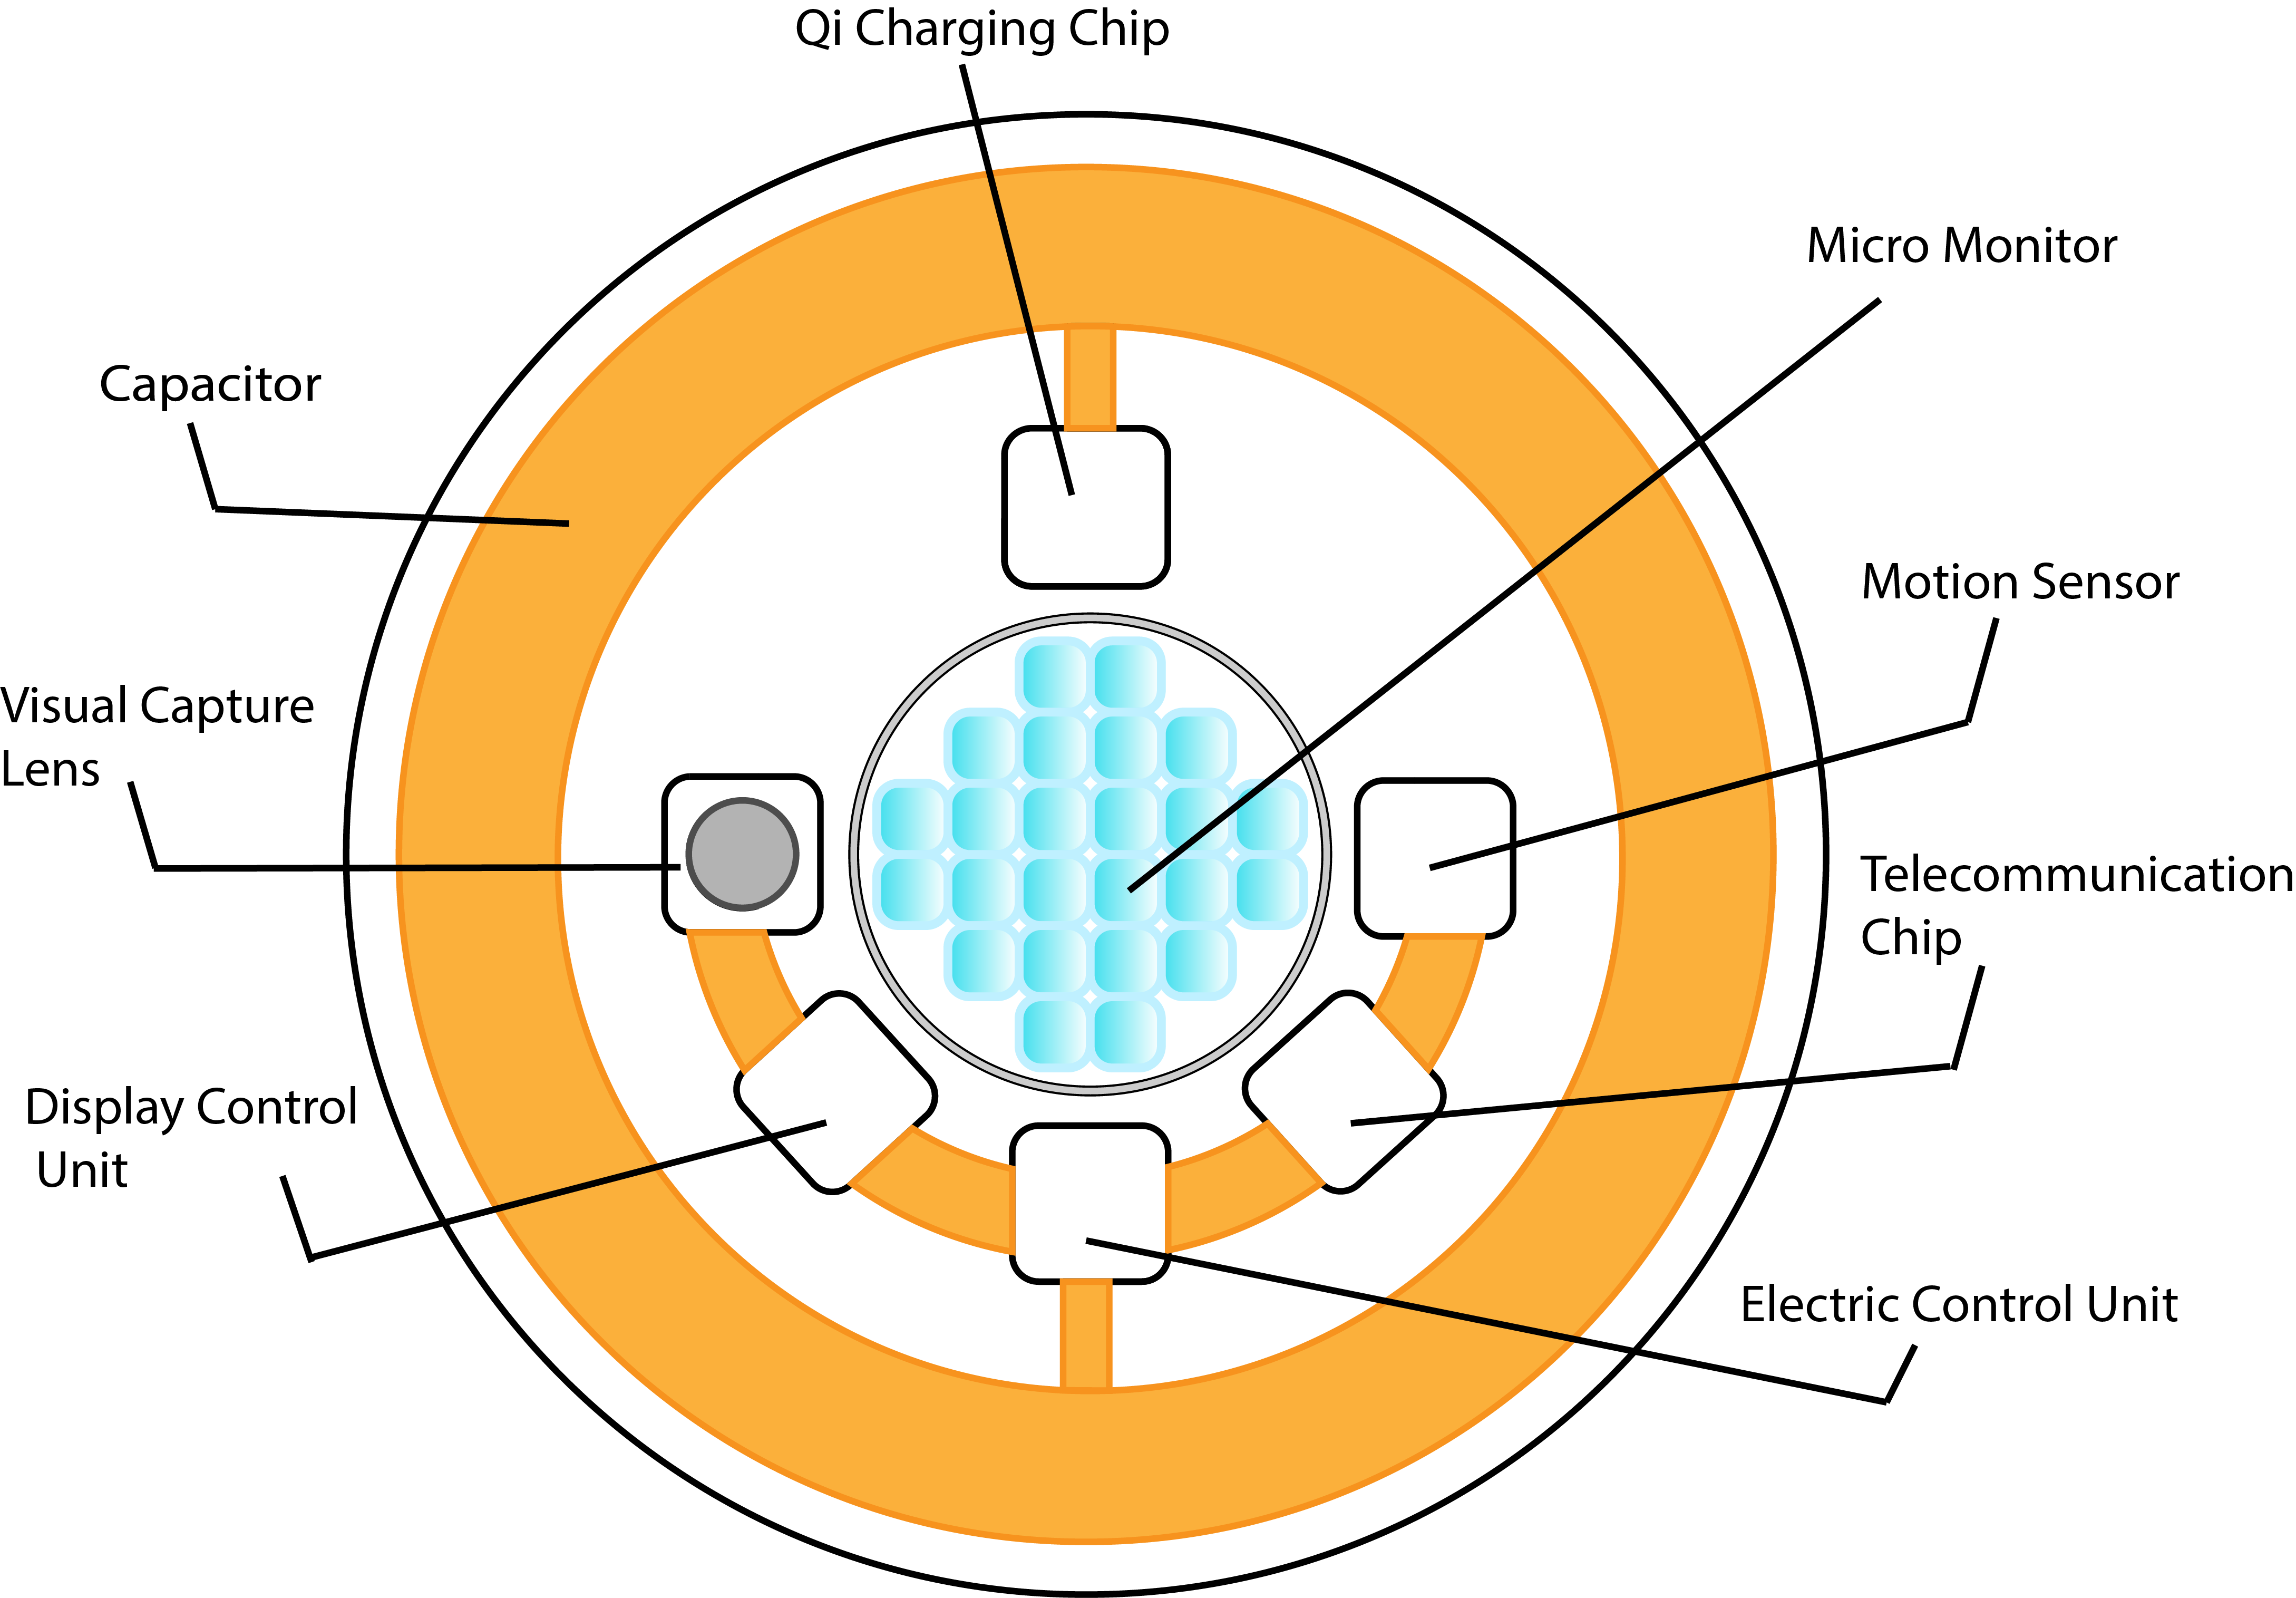
\includegraphics[width=\columnwidth]{NaviLens_Lens.png}
 \caption{NaviLens}
 \label{fig:NaviLens}
\end{figure}

\subsection{NaviLens Multifunction Case}

The NaviLens Multifunction Casing is the protective device that stores the NaviLens when it is not in use, and it protects the NaviLens from broken or become dirty. When using the case, refill the Contact Lens solution to keep NaviLens moisture and clean. The case is built-in with ultrasonic cleaning technology which helps provide a thorough cleaning process and sterilize the lens. Under the notch of the case, there contains two wireless charging pad which use to charge the NaviLens. The case has a  Micro-USB Type C port for charging and cleaning purpose.\\


\begin{figure}
 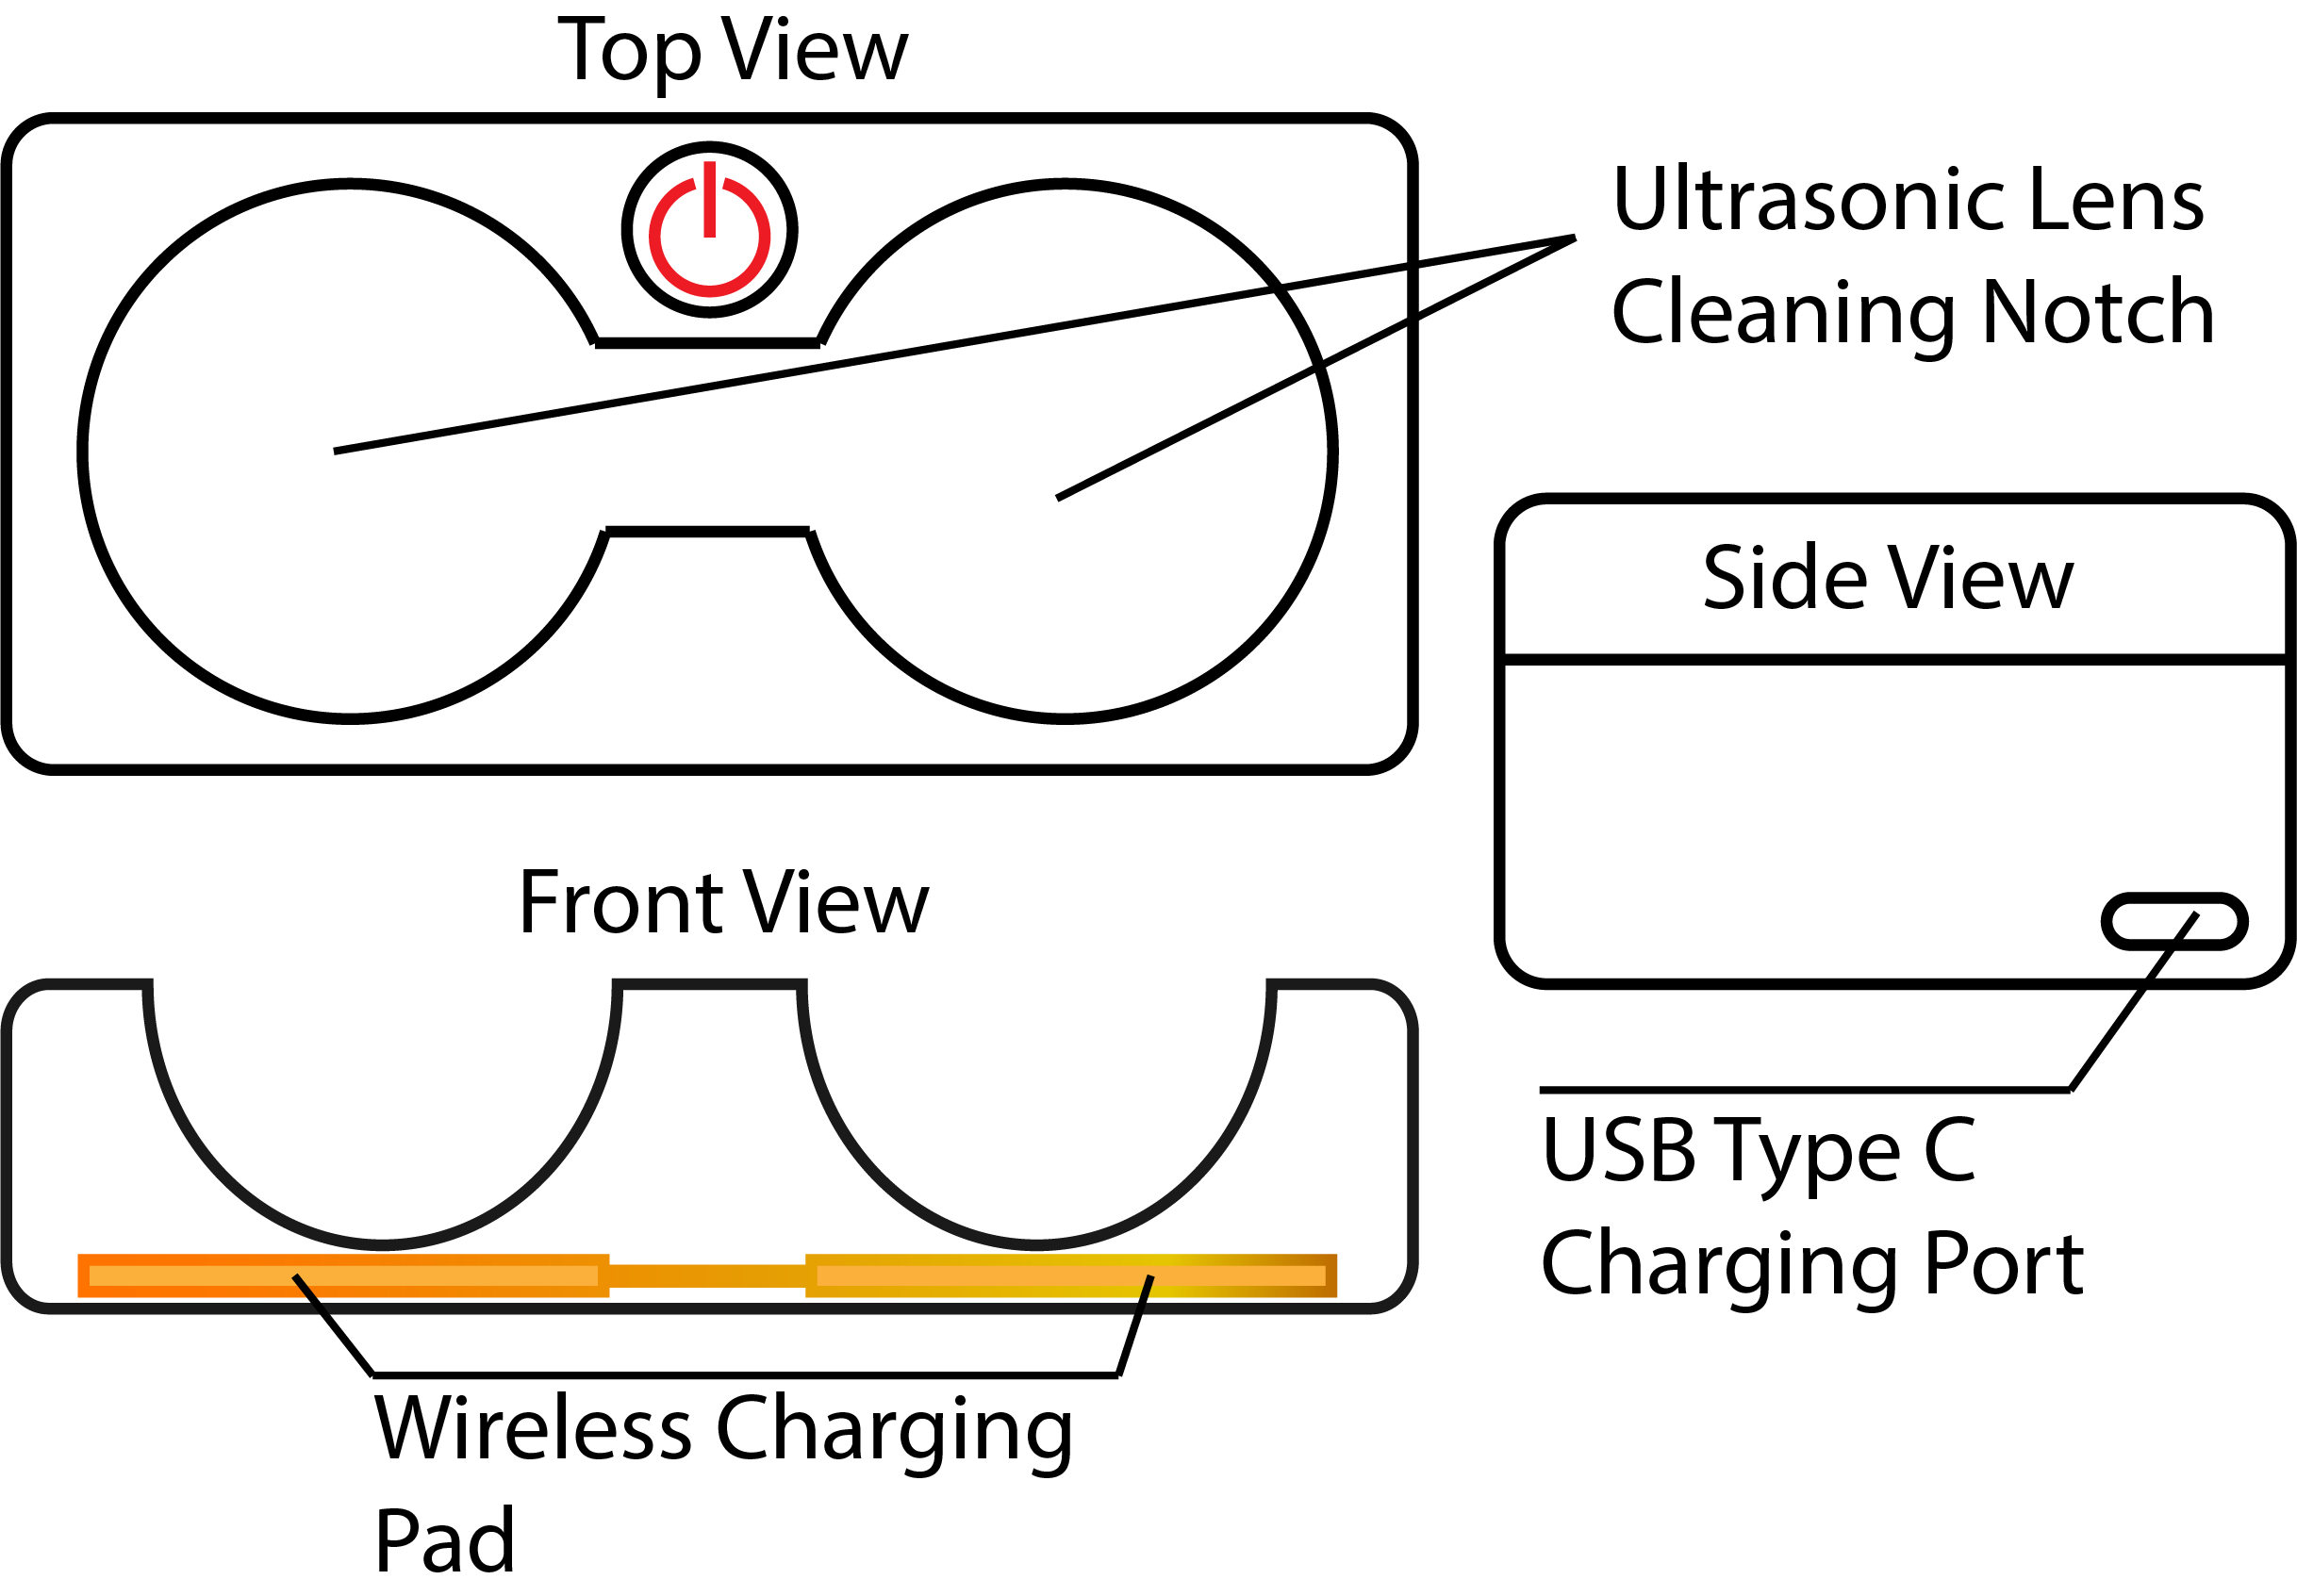
\includegraphics[width=\columnwidth]{Casing.png}
 \caption{NaviLens Casing}
 \label{fig:Casing}
\end{figure}

\subsection{Global Positioning System}

\begin{figure}
 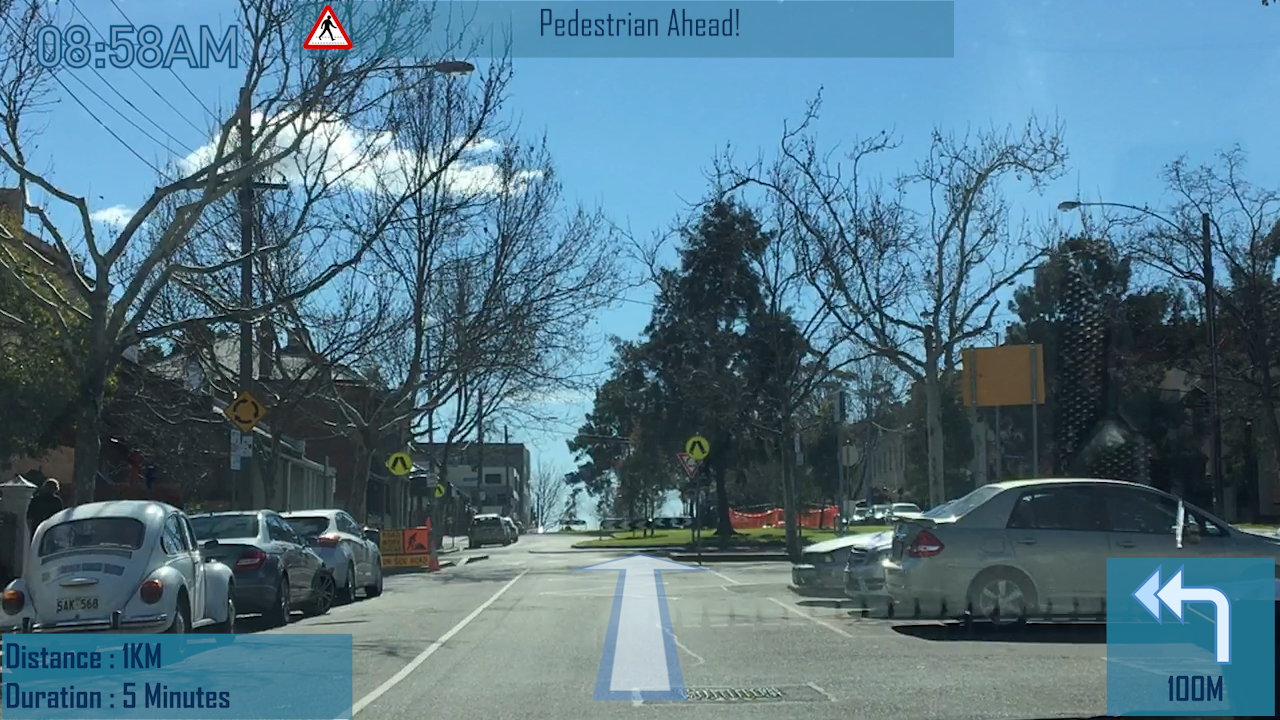
\includegraphics[width=\columnwidth]{gui.png}
 \caption{Navigation HUD Design}
 \label{fig:gui}
\end{figure}

Through the survey, we found that more and more drivers were relying on the road navigation application on their mobile phone or built-in navigation device in their car. Besides, the survey also showed that the percentage of car accident increased which might be caused by distraction from staring at the mobile phone or the multimedia monitor in their car and cause leaving the eyesight on the road while driving. From the obsession above, the main aim of NaviLens was to achieve a state that drivers always focused their eyesight on the road and remove any distraction caused by mobile phone or car multimedia monitor while driving. From the past, most of the navigation information was notified by sound and visual on the device. However, when the notification message was too vague, this caused the driver to check their device while still driving on the road.\\

As a wearable accessory that supported on eye vision sensor, NaviLens contained a set of micro-monitors that showed navigation path directly on top. To activate the navigation function on NaviLens, drivers first input their destination through the application on their mobile phone, then the navigation information started showing on the micro-monitor on the NaviLens. To make the navigation details precisely, whenever the drivers reached the complicated crossroad or split road, the built-in camera of NaviLens could detect the road markings and project the navigation path in between those markings on the road. This integration decreased the misleading of the uncertainty navigation information and highly decreased the chance of an accident caused by distraction while driving on the road.\\

\subsection{Signboard attention}
When driving on roads, there was a lot of things that drivers needed to notice with, and sometimes drivers might miss some of the important signboards on the side of the road, such as the speed limit sign or pedestrian road sign board. This kind of mistake might lead to the chance of an accident to increase as well as cause life risk to the pedestrian.\\

So, the built-in camera of NaviLens streamed the visual image to the application on the phone and processed the image to detect those signboards. Once the application detected the signboard, it showed a notice frame around those signs on NaviLens to notify drivers. Once the driver saw it, the sensor of NaviLens could detect the motion of eye turning and make the frame disappear for letting the driver focus driving on the road.\\

\subsection{Eye sightedness and Colour blindness}

Some persons were born naturally with color blindness while the most common types of color blindness were red-green color blindness, blue-yellow color blindness, and complete color blindness. However, since NaviLens was a technology that focuses on the road safety, we focused more on red-green color blindness person as to identify the color scheme of the traffic lights. Based on terms, red-green color blindness persons won’t be able to identify the color of red and green probably, and this could lead to a lot of crisis, for example, they were unable to identify the traffic lights while crossing the road or stopped the car immediately while reaching the crossroad. Although these kinds of person were encouraged not to drive on the road, with the release of NaviLens, the technology could support more and more color blindness persons to be in touch with transport and traffic safeness.\\

Besides, NaviLens also help the eye sightedness person to adjust their eyesight like the traditional contact lenses. The structure of NaviLens had two parts, the front part was the eye sickness correction section, and the back part was the electronic board integration area. The combination of the front section could be switched easily by professional optical shop or clinic. Before purchasing the NaviLens, a person should have their eye checked and had the best combination which best suited their eyes condition and depended on their needs. If the combination needed to be changed in future, simply returned to the shop or clinic and switched the front section.\\

\begin{figure}
 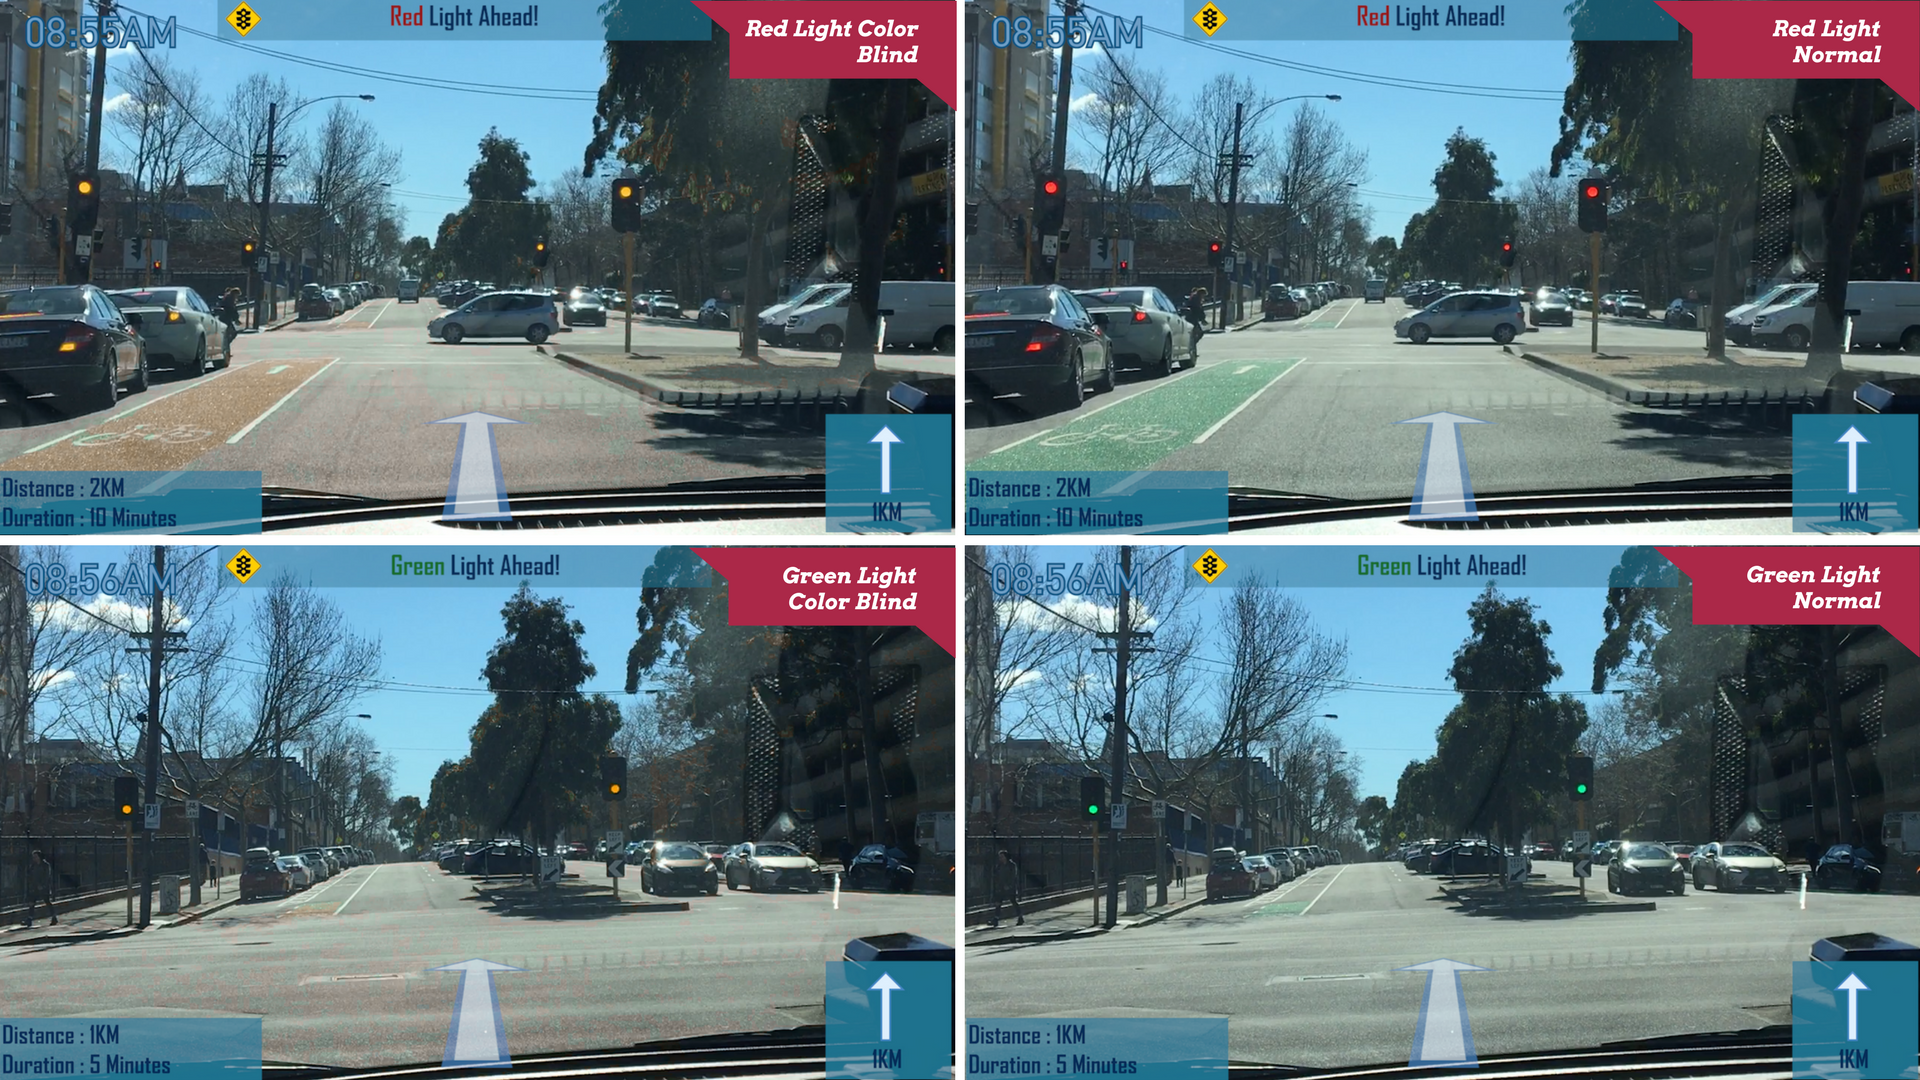
\includegraphics[width=\columnwidth]{colorblindess.png}
 \caption{Normal and Color Blindness}
 \label{fig:colorblindess}
\end{figure}

\subsection{Driving Enforcement Marking System}

NaviLens was a product that co-partnership of Australia Department of Transport and Insurance Australia Group. We implemented a feature that could help capture the driving offences through the built-in camera of NaviLens. With the help of captured visual evidence, police could make a punishment to the driver based on the car plate details and the offences performed. Besides, insurance fee on the current car might also increase for further insurance purpose.\\

Whenever the driver was driving, the NaviLens would capture all the information of the context which was within the range of the eyesight. The information captured contained car plate, the location and time information. Once the NaviLens detected an offence was performed by one of the cars within the capture stream, NaviLens would record the information and sent it to the police and insurance company. The database system would save all the records and perform the punishment automatically based on the information. If the same relevant records were captured simultaneously, the system would only perform one punishment for the record. The message would be sent to the driver as well as insurance company after the punishment has been recorded. If the driver had any disagreement for the offense, the officer could retrieve the detail and provided a second review of the record.\\


\begin{figure}
\centering
 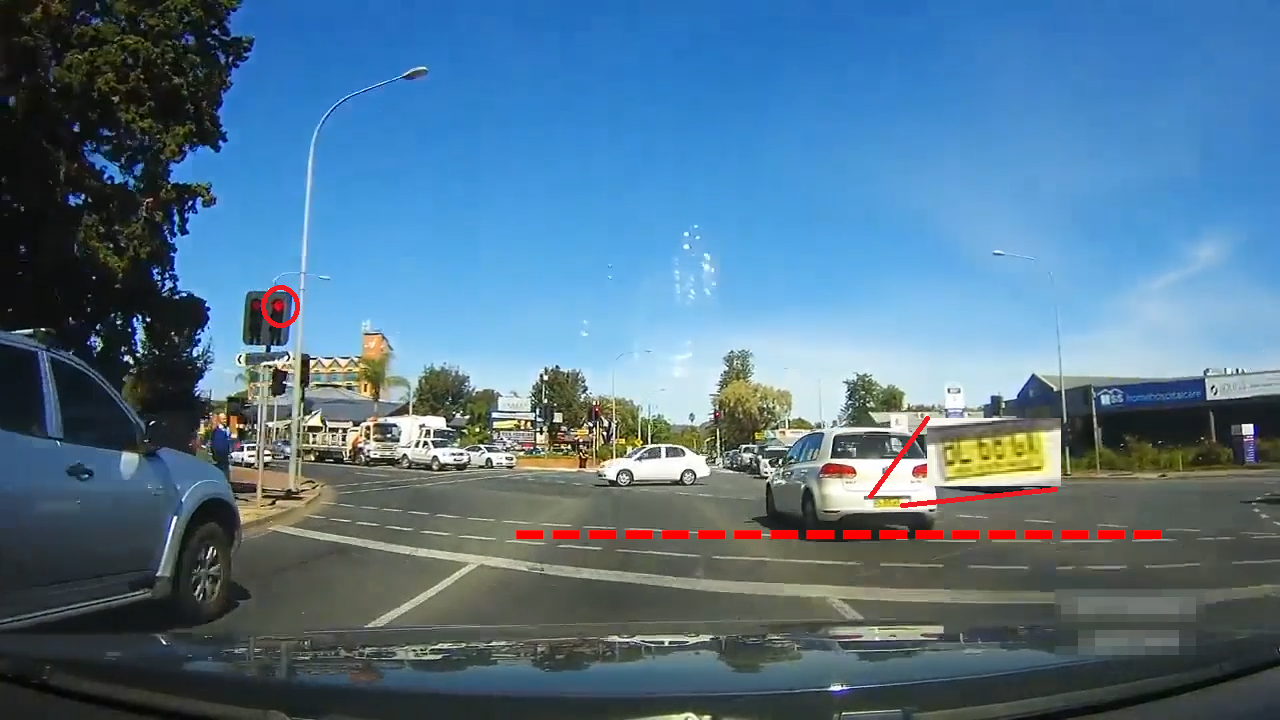
\includegraphics[width=0.7\columnwidth]{illegal.png}
 \caption{Illegal Action Captured}
 \label{fig:illegal}
\end{figure}

\begin{figure}
\centering
 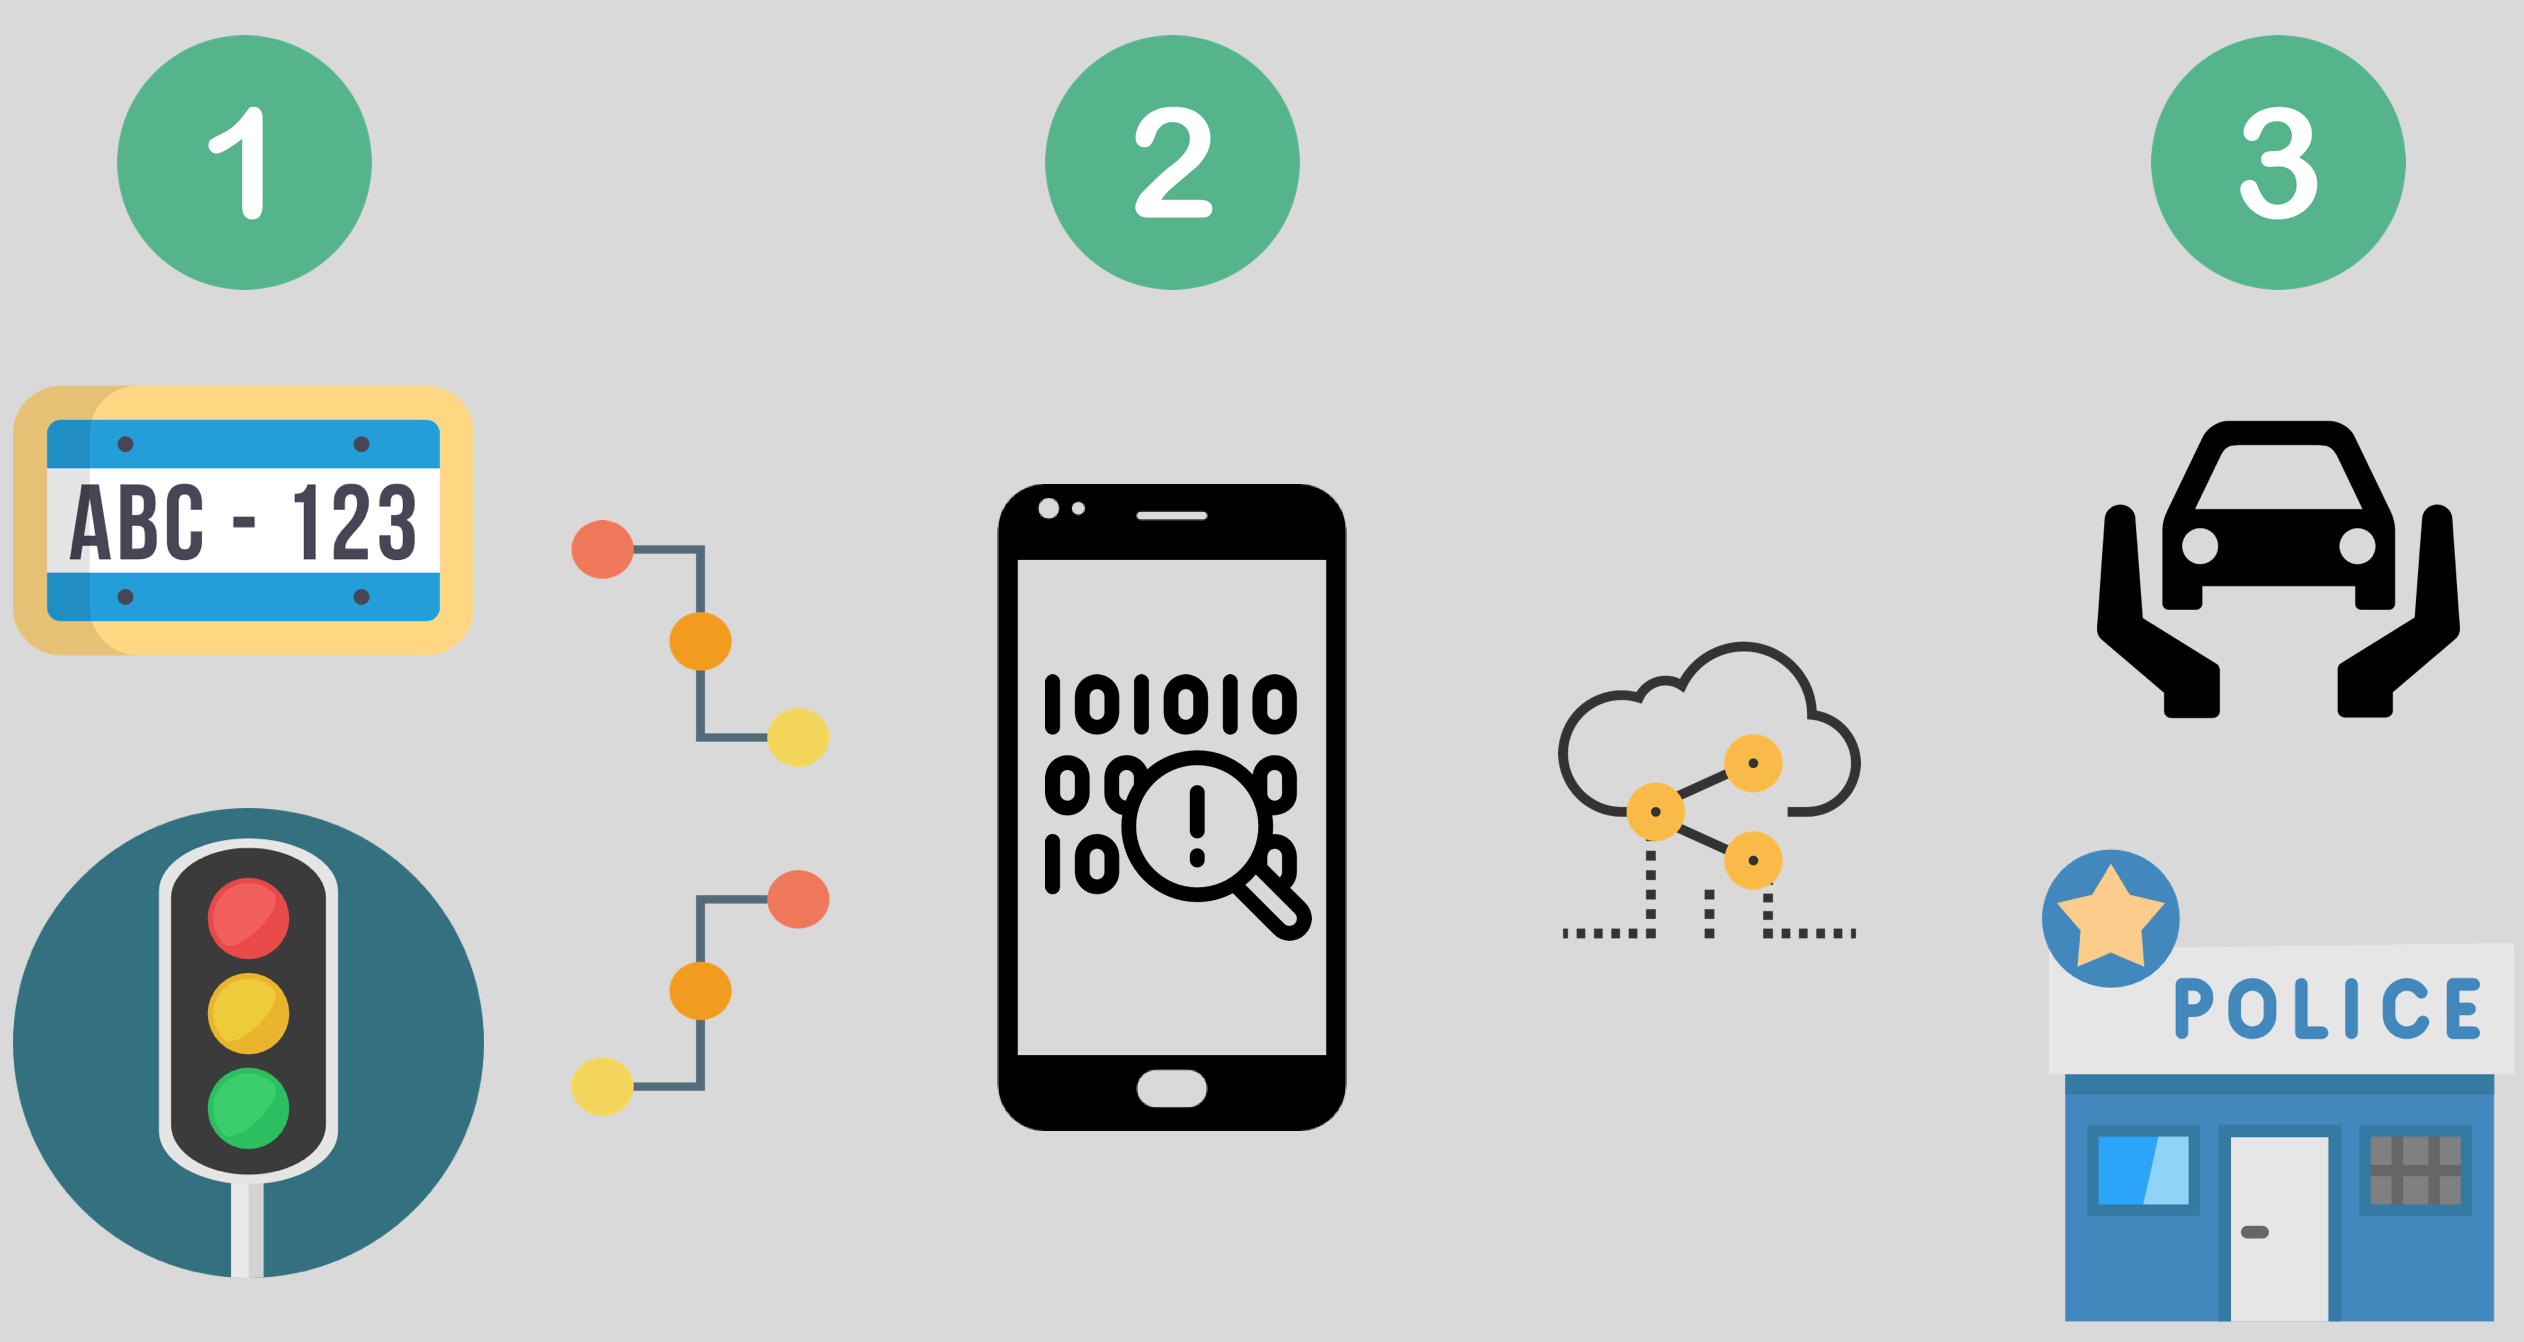
\includegraphics[width=0.7\columnwidth]{datatransform.png}
 \caption{Record Uploaded to Database}
 \label{fig:datatransform}
\end{figure}

\subsection{Lens Trial}
\emph{Driving Enforcement Marking System}\\
The aim of trial was to evaluate the system's telecommunication, infrastructure, and generate deep insights into the feasibility and accuracy of system's marking criteria.\\

We run the trial of driving enforcement system in a closed proving ground, which had a boundary of 5km, authorized by the Department of Transport. This place was chosen specifically as it had essential components, such as traffic light, traffic lane, sidewalk line, and roundabout, etc. to simulate actual traffic environment. The trial lasted three hours in total: 1.5 hours during day time and 1.5 hours during night, so that we could evaluate how well the system captured the image under different luminous intensity.\\

We recruited ten participants (four female) who were eligible for driving and wearing the contact lens to drive as normal. We hired 10 testing cars and motorbikes (installed with specifically designed safety devices) which were labeled with distinctive warning sign from Department of Transport for the participants. Especially, considering the safety issue, two of the participants were trained professional drivers, they were told to drive as normal, but deliberately perform driving offenses on occasion during the trial. All the driving offenses were fully video recorded by our observer for further review.\\

During the trial, the other eight participants wore the contact lens to capture the image on their way and the driving offenses were recognized automatically through our unique algorithm. We gathered several types of data in order to assess the marking system's usability and effectiveness. This includes the actual list of driving offenses performed and their frequency (run the red light, over-speeding and change the lane without turning on signal etc) as well as the related image captured and an analysis result recognized by the system. We processed these data to primarily focus on the quality of identification of ‘driving offenses’: precision of each type of offenses identified; recall of each type of offenses identified; influence from the luminous intensity. In addition to the default setup in the system, we also encouraged the participants to propose any driving actions they considered ‘improper’ to contribute improvement to system's applicability and generality.\\

Figure 3 and 4 illustrated the results about how well the systems recognized the top twelve driving offenses in term of precision and recall, both in day time and night. These resignations of driving defenses were verified by qualified officers from Department of Transport. The trial results showed that the system achieved a high precision in recognizing driving defenses with over 98\% in average. The recall data had a significant decrease especially in recognizing the offenses of not wearing safety belts, talking on cell phone and not using helmets at night due to the light reflected from the front windshield.\\

To access the appeal of comfortableness of wearing the lens, we did not specify how long the NaviLens should be worn during the trial, so long as participants could use the lens for a minimum of 30 minutes per day, and did not feel the discomfort of eyes. Whilst the system's precision and recall were considerable and there was some room for improvement in night recognition, the trial results indicated that the system was accepted by Department of Transport, and participants felt it enjoyable as they were providing an important role in keeping the road more safety.\\


\begin{figure}
\centering
 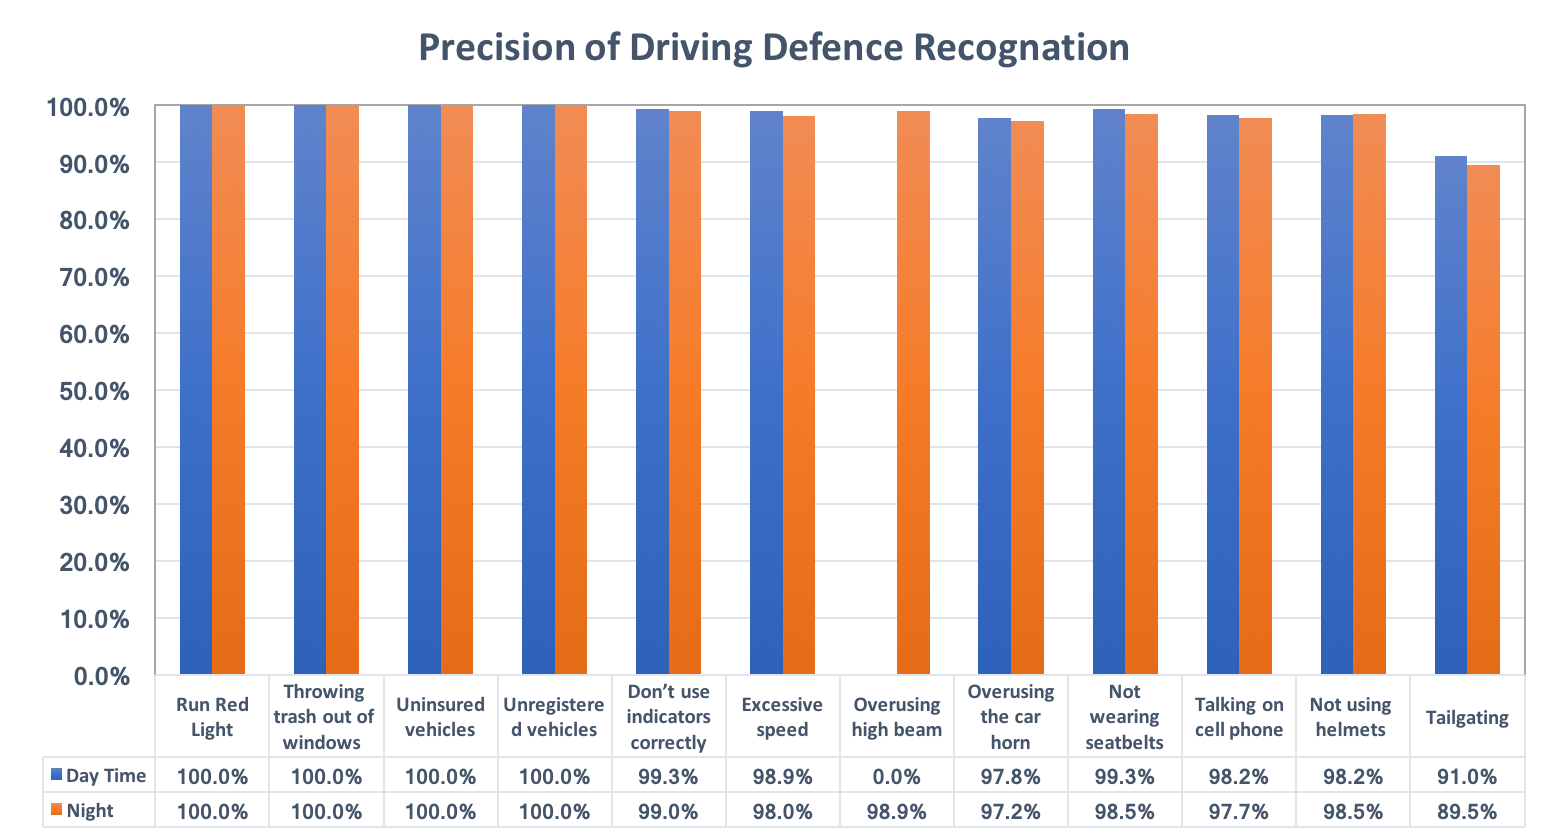
\includegraphics[width=0.8\columnwidth]{Precision.png}
 \caption{Recognition precision of driving offences }
 \label{fig:Precison}
\end{figure}

\begin{figure}
\centering
 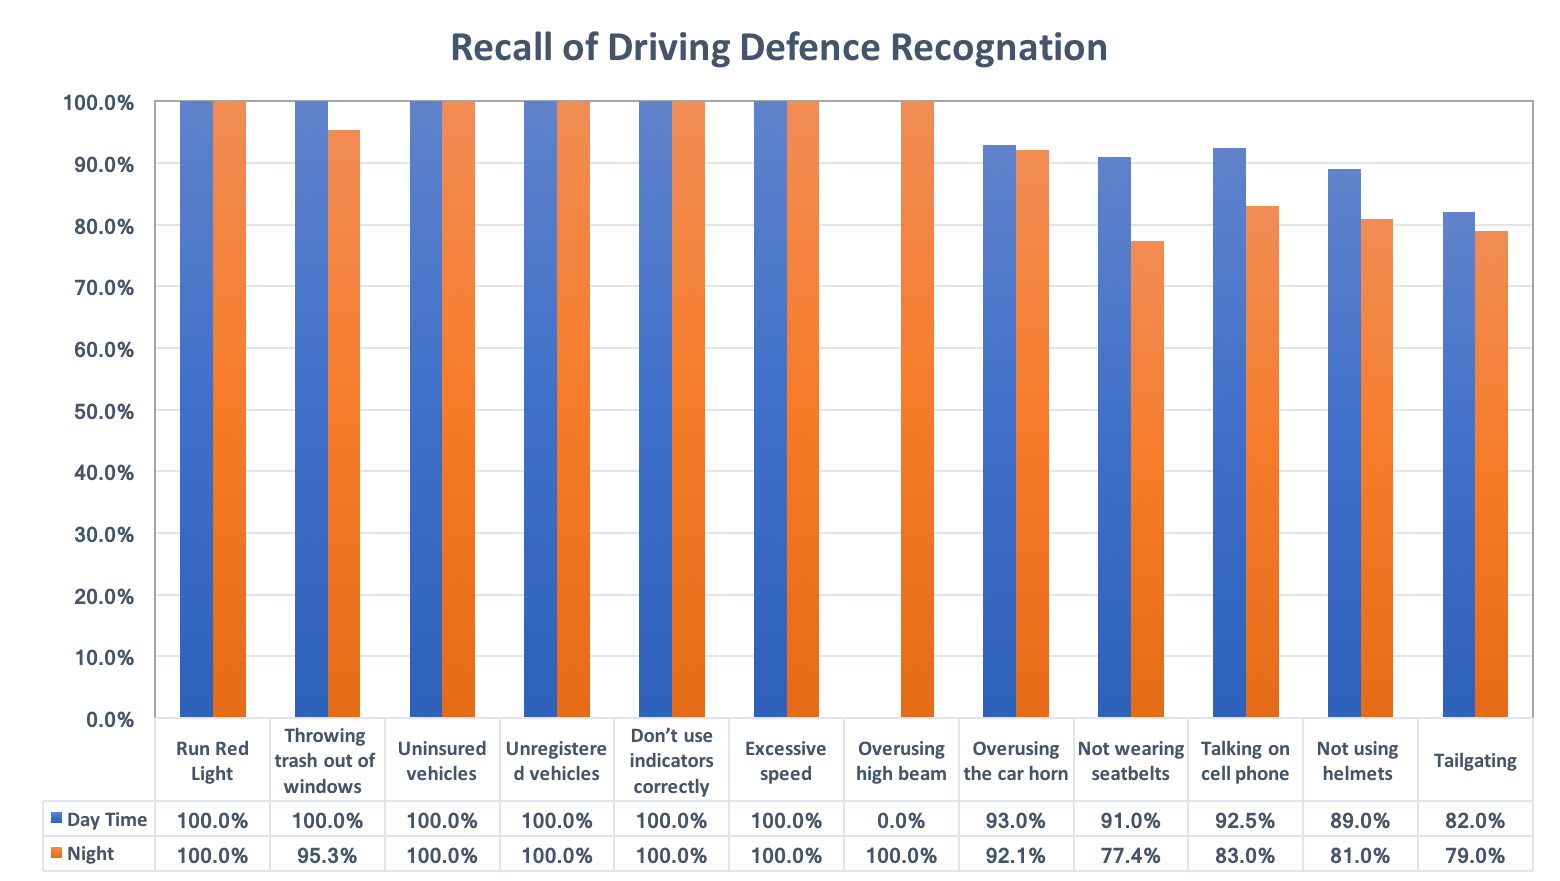
\includegraphics[width=0.8\columnwidth]{recall.png}
 \caption{Recognition recall of driving offences }
 \label{fig:recall}
\end{figure}

\emph{Navigation}\\
The aim of the trial was to evaluate how well the navigation shown by lens went along with the actual Google Map direction, and how the system helped driver concentrate on driving.\\

Twenty participants (8 female, 2 red blindness), between 1 to 20 driving years, joined in this trial. Half of them wore the NaviLens for navigation during their driving while the rest used mobile phone. We installed a video camera in their own car to record how they interacted with different navigation device during driving and whether they concentrate more on the traffic. In addition, the NaviLens recorded all the scene shown to the driver, and we reviewed these data to see if had NaviLens detected signboards correctly for drivers and traffic lights for red blindness participants.\\

This trial lasted one week, and trial participants were required to wore NaviLens for navigation whenever they drove. We did not limit the driving area and encouraged the participants to drive to some remote areas with weak GPS signal or areas with complex road conditions to test the feasibility of the system. They were also encouraged to keep daily reflective logs and were required to attend a half day debrief discussion session at the end of the trial. We improved the NaviLens interface by adding or removing features, adjusting manifestation mode etc based on participants' feedback, as shown in the screenshot (Figure 7).\\

The Figure 12 illustrated the statistical data about how frequency the participants took their eyes off the road during a certain period of driving. It showed that the participants who wore NaviLens concentrated more on checking traffic than the ones using mobile phone or vehicle navigation.\\

\begin{figure}
 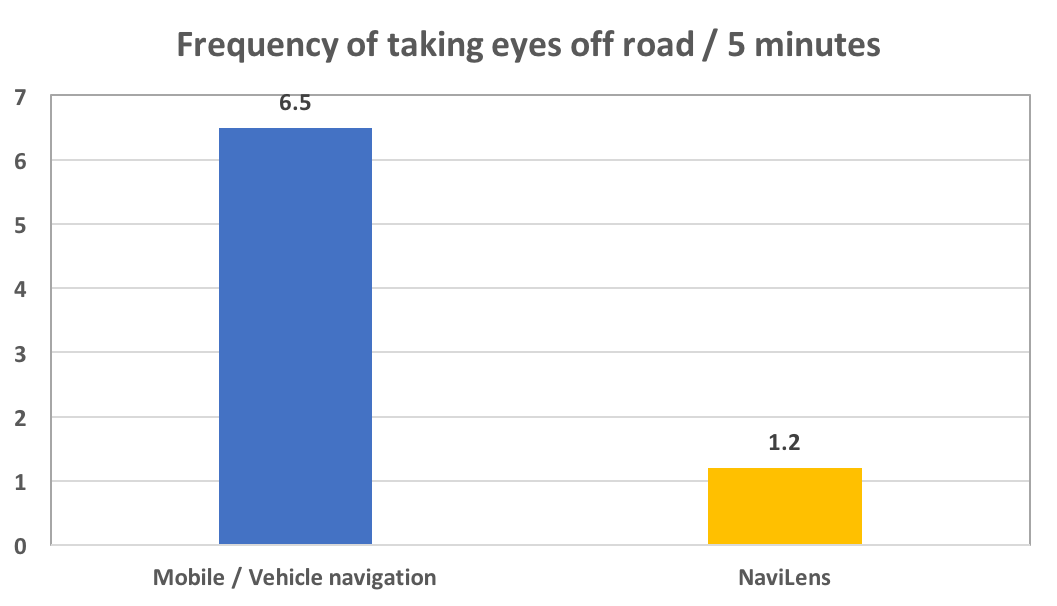
\includegraphics[width=\columnwidth]{eyesOff.png}
 \caption{Frequency of taking eyes off road}
 \label{fig:eyesOff}
\end{figure}

\subsection{Conclusion}
Based on our trial, we have noticed that NaviLens can help us reduce dependence on mobile devices and better regulate the driving behavior, it helps people concentrate on the road conditions and reduces the risk of accidents. The research in this paper and the related artifacts are part of the design fiction, however, along with the perfection of functions, it will enable active decision-making for a safer future.\\

\nocite{ref1}
\nocite{ref2}
\nocite{ref3}
\nocite{ref4}
\nocite{ref5}
\nocite{ref6}

\bibliography{papers}
\bibliographystyle{abbrv}

\end{multicols}

\end{document}